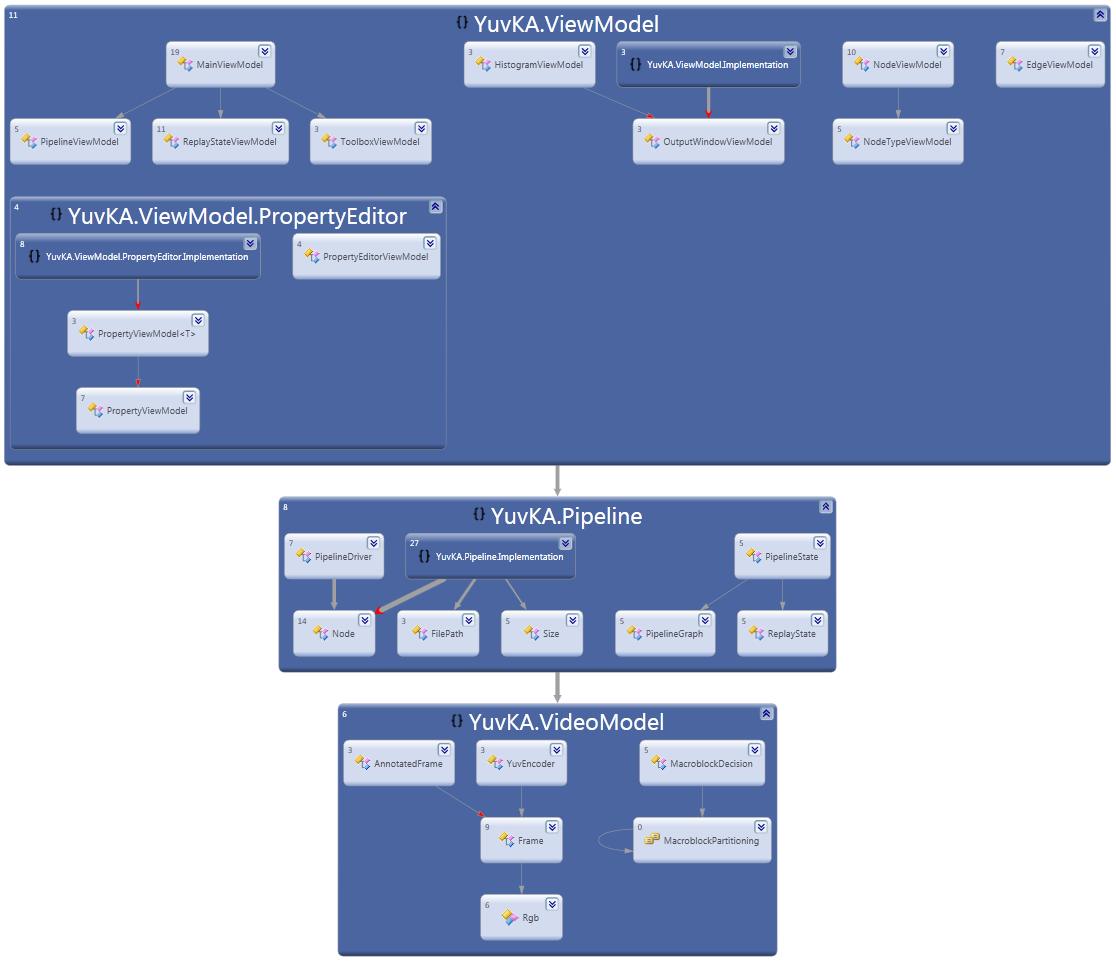
\includegraphics[width=\textwidth]{Diagrams/namespacedependencies.png}
Veranschaulichung der MVVM\footnote{\emph{Model-View-ViewModel}}-Architektur, die bei diesem Projekt umgesetzt wird. Die View wird hierbei jedoch nicht dargestellt, da sie selbst keinerlei Logik enthält.
\begin{description}
	\item[YuvKA.VideoModel]~\\
	Das VideoModel repräsentiert ein eingelesenes Video, ggf. mit zugehörigen Log-Daten. Da es die Daten im RGB-Format speichert, müssen diese bei Eingabe und Ausgabe von einem YUV-Encoder konvertiert werden.

	\item[YuvKA.Pipeline]~\\
	Die Pipeline-Schicht repräsentiert den UI-unabhängigen Aufbau des Analyse-DAGs\footnote{\emph{directed acyclic graph}}. Sie besteht einerseits aus den unterschiedlichen Knoten-Klassen, die unabhängig voneinander ihren jeweiligen Algorithmus auf Frame-für-Frame-Basis implementieren, und andererseits aus dem Pipeline Driver, der für die Abhängigkeitsauflösung und letztendliche Abarbeitung der Pipeline zuständig ist.

	\textbf{YuvKA.Pipeline.Implementation:} Namespace der vordefinierten Knotentypen. Diese werden dynamisch bei Programmstart ermittelt und geladen.
	
	\item[YuvKA.ViewModel]~\\
	Nach dem MVVM-Pattern ist es Aufgabe der ViewModel-Schicht, der View das Model in einer für sie verarbeitbaren Form zu präsentieren. Bezogen auf das Projekt bedeutet dies vor allem, die Model-Klassen um View-spezifische Daten und Methoden zu ergänzen.

	\textbf{YuvKA.Pipeline.ViewModel.Implementation:} Namespace der ViewModels der vordefinierten Knotentypen.
	
	\item[YuvKA.ViewModel.PropertyEditor]~\\
	Die Klassen des PropertyEditor-Namespaces erzeugen für ein beliebiges Objekt dynamisch eine Oberfläche zum Anzeigen und Ändern seiner Property-Werte. Die Menge der darstellbaren Property-Typen ist dynamisch erweiterbar.

	\textbf{YuvKA.ViewModel.PropertyEditor.Implementation:} Namespace der vordefinierten Property-Typen.

\end{description}



